\documentclass{beamer}
\mode<presentation> {
%\usetheme{Madrid}
%\usetheme{default}
\usepackage{color}
\definecolor{bottomcolour}{rgb}{0.21,0.11,0.21}
\definecolor{middlecolour}{rgb}{0.21,0.11,0.21}
\setbeamercolor{structure}{fg=white}
\setbeamertemplate{frametitle}[default]%[center]
\setbeamercolor{normal text}{bg=black, fg=white}
\setbeamertemplate{background canvas}[vertical shading]
[bottom=bottomcolour, middle=middlecolour, top=black]
\setbeamertemplate{items}[circle]
\setbeamertemplate{navigation symbols}{} %no nav symbols
\setbeamercolor{block title}{use=structure,fg=white,bg=structure.fg!50!red!50!blue!100!green}
\setbeamercolor{block body}{parent=normal text,use=block title,bg=block title.bg!5!white!10!bg,fg=white}
\setbeamertemplate{navigation symbols}{}
}

\usepackage{graphicx} 
\usepackage{booktabs} 
\usepackage[utf8]{inputenc}  
\usepackage[T1]{fontenc}  
\usepackage{geometry}     
\usepackage[francais]{babel} 
\usepackage{eurosym}
\usepackage{verbatim}
\usepackage{ragged2e}
\justifying


%%%%%%%%%%%%%%%%%%%%%%%%%%%%%%%%%%%%%%%%%%%%%%%%%%%%%%%%%%%%%%%%
%% ccBeamer 0.1, 2007-07-02                                   %%
%% Written by Sebastian Pipping <webmaster@hartwork.org>      %%
%% ---------------------------------------------------------- %%
%% Licensed under Creative Commons Attribution-ShareAlike 3.0 %%
%% http://creativecommons.org/licenses/by-sa/3.0/             %%
%%%%%%%%%%%%%%%%%%%%%%%%%%%%%%%%%%%%%%%%%%%%%%%%%%%%%%%%%%%%%%%%


%% Images
\newcommand{\CcImageBy}[1]{%
	
\includegraphics[scale=#1]{creative_commons/cc_by_30.pdf}%
}
\newcommand{\CcImageCc}[1]{%
	
\includegraphics[scale=#1]{creative_commons/cc_cc_30.pdf}%
}
\newcommand{\CcImageDevNations}[1]{%
	
\includegraphics[scale=#1]{creative_commons/cc_dev_nations_30.pdf}%
}
\newcommand{\CcImageNc}[1]{%
	
\includegraphics[scale=#1]{creative_commons/cc_nc_30.pdf}%
}
\newcommand{\CcImageNd}[1]{%
	
\includegraphics[scale=#1]{creative_commons/cc_nd_30.pdf}%
}
\newcommand{\CcImagePd}[1]{%
	
\includegraphics[scale=#1]{creative_commons/cc_pd_30.pdf}%
}
\newcommand{\CcImageSa}[1]{%
	
\includegraphics[scale=#1]{creative_commons/cc_sa_30.pdf}%
}
\newcommand{\CcImageSampling}[1]{%
	
\includegraphics[scale=#1]{creative_commons/cc_sampling_30.pdf}%
}
\newcommand{\CcImageSamplingPlus}[1]{%
	
\includegraphics[scale=#1]{creative_commons/cc_sampling_plus_30.pdf}%
}


%% Groups
\newcommand{\CcGroupBy}[1]{% zoom
	\CcImageBy{#1}%
}
\newcommand{\CcGroupByNc}[2]{% zoom, gap
	\CcImageBy{#1}\hspace*{#2}\CcImageNc{#1}%
}
\newcommand{\CcGroupByNcNd}[2]{% zoom, gap
	\CcImageBy{#1}\hspace*{#2}\CcImageNc{#1}\hspace*{#2}\CcImageNd{#1}%
}
\newcommand{\CcGroupByNcSa}[2]{% zoom, gap
	\CcImageBy{#1}\hspace*{#2}\CcImageNc{#1}\hspace*{#2}\CcImageSa{#1}%
}
\newcommand{\CcGroupByNd}[2]{% zoom, gap
	\CcImageBy{#1}\hspace*{#2}\CcImageNd{#1}%
}
\newcommand{\CcGroupBySa}[2]{% zoom, gap
	\CcImageBy{#1}\hspace*{#2}\CcImageSa{#1}%
}
\newcommand{\CcGroupDevNations}[1]{% zoom
	\CcImageDevNations{#1}%
}
\newcommand{\CcGroupNcSampling}[2]{% zoom, gap
	\CcImageNc{#1}\hspace*{#2}\CcImageSampling{#1}%
}
\newcommand{\CcGroupPd}[1]{% zoom
	\CcImagePd{#1}%
}
\newcommand{\CcGroupSampling}[1]{% zoom
	\CcImageSampling{#1}%
}
\newcommand{\CcGroupSamplingPlus}[1]{% zoom
	\CcImageSamplingPlus{#1}%
}


%% Text
\newcommand{\CcLongnameBy}{Attribution}
\newcommand{\CcLongnameByNc}{Attribution-NonCommercial}
\newcommand{\CcLongnameByNcNd}{Attribution-NoDerivs}
\newcommand{\CcLongnameByNcSa}{Attribution-NonCommercial-ShareAlike}
\newcommand{\CcLongnameByNd}{Attribution-NoDerivs}
\newcommand{\CcLongnameBySa}{Attribution-ShareAlike}

\newcommand{\CcNote}[1]{% longname
	This work is licensed under the \textit{Creative Commons #1 3.0 License}.%
}


\title[Thunderbird et clefs PGP]{Thunderbird et clefs PGP} 
\author{Genma}

\begin{document}

%% Titlepage
\begin{frame}
	\titlepage
	\vfill
	\begin{center}
		\CcGroupByNcSa{0.83}{0.95ex}\\[2.5ex]
		{\tiny\CcNote{\CcLongnameByNcSa}}
		\vspace*{-2.5ex}
	\end{center}
\end{frame}


%\begin{frame}
%\frametitle{Plan} 
%\tableofcontents
%\end{frame}

%----------------------------------------------------------------------------------------
%	PRESENTATION SLIDES
%----------------------------------------------------------------------------------------


\begin{frame}
\frametitle{
\includegraphics[scale=0.4]{./Genma.jpg} \ \ \  A propos de moi  }
\begin{columns}[c] 

\column{.55\textwidth} 
\textbf{Où me trouver sur Internet?}
\begin{itemize}
\item Le Blog de Genma : http://genma.free.fr
\item Twitter : http://twitter.com/genma
\end{itemize}

\textbf{Mes centres d'intérêts?}
\\ Plein de choses dont:
\begin{itemize}
\item La veille technologique
\item Le chiffrement
\end{itemize}

\column{.5\textwidth} 
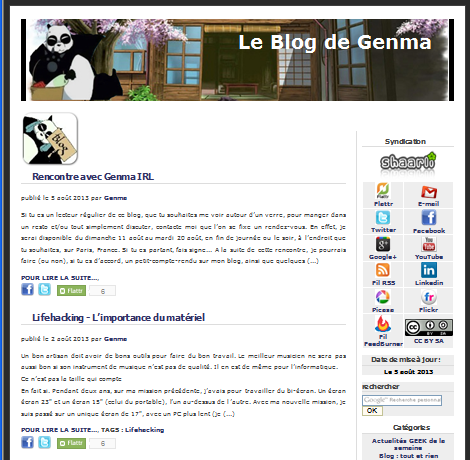
\includegraphics[width=5cm,height=5cm]{blog.png} 

\end{columns}
\end{frame}


%----------------------------------------------------------------------------------------
\begin{frame}
\frametitle{Thunderbird - enigmail}
\begin{itemize}
\item Dans Thunderbird, il suffit d'ajouter l'extension Enigmail.
\end{itemize}
\begin{center}

\includegraphics[scale=0.5] {./images/Thunderbird_Extension_Enigmail.png}
\end{center}
\end{frame}


%----------------------------------------------------------------------------------------
\begin{frame}
\begin{center}
\Huge{Enigmail - l'assistant}
\end{center}
\end{frame}

%----------------------------------------------------------------------------------------
\begin{frame}
\frametitle{Enigmail - l'assistant}
\begin{center}
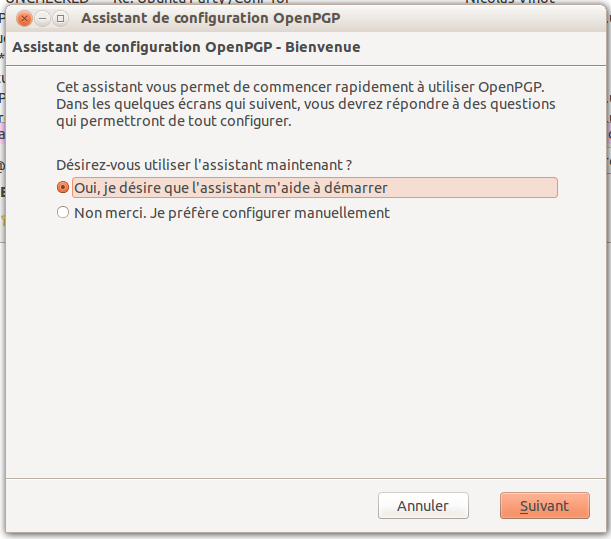
\includegraphics[scale=0.3] {./images/Assistant01.png}
\end{center}
\end{frame}

%----------------------------------------------------------------------------------------
\begin{frame}
\frametitle{Enigmail - l'assistant}
\begin{center}
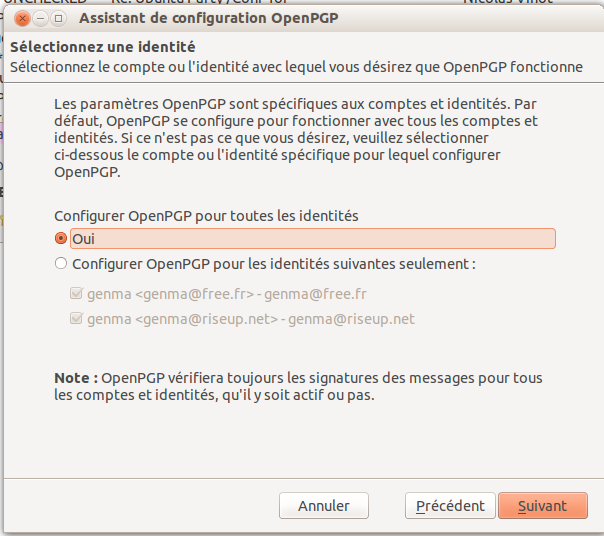
\includegraphics[scale=0.3] {./images/Assistant02.png}
\end{center}
\end{frame}

%----------------------------------------------------------------------------------------
\begin{frame}
\frametitle{Enigmail - l'assistant}
\begin{center}
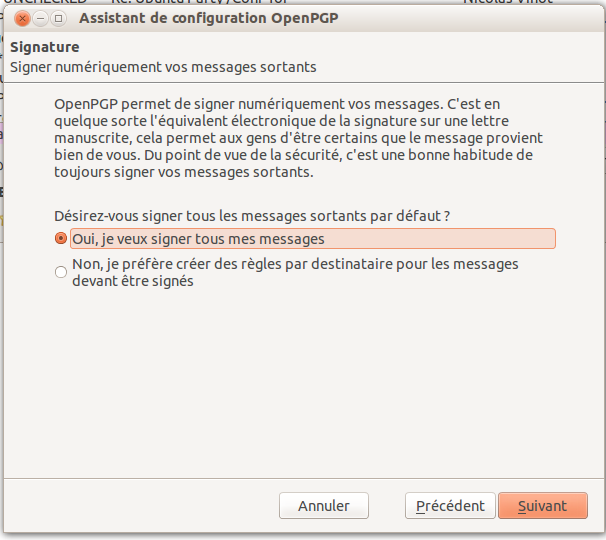
\includegraphics[scale=0.3] {./images/Assistant03.png}
\end{center}
\end{frame}

%----------------------------------------------------------------------------------------
\begin{frame}
\frametitle{Enigmail - l'assistant}
\begin{center}
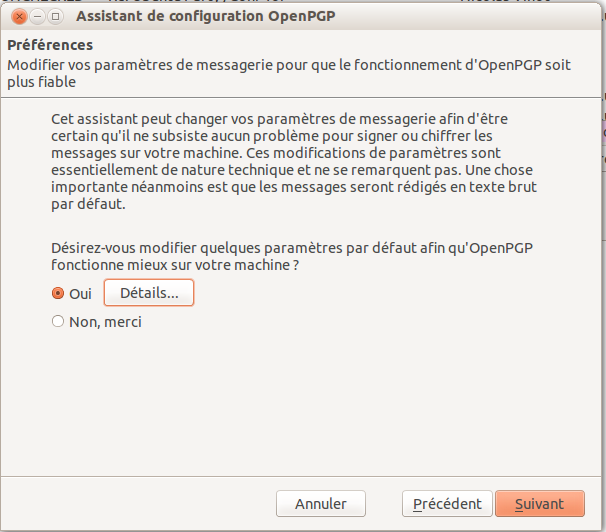
\includegraphics[scale=0.3] {./images/Assistant04.png}
\end{center}
\end{frame}

%----------------------------------------------------------------------------------------
\begin{frame}
\frametitle{Enigmail - l'assistant}
\begin{center}
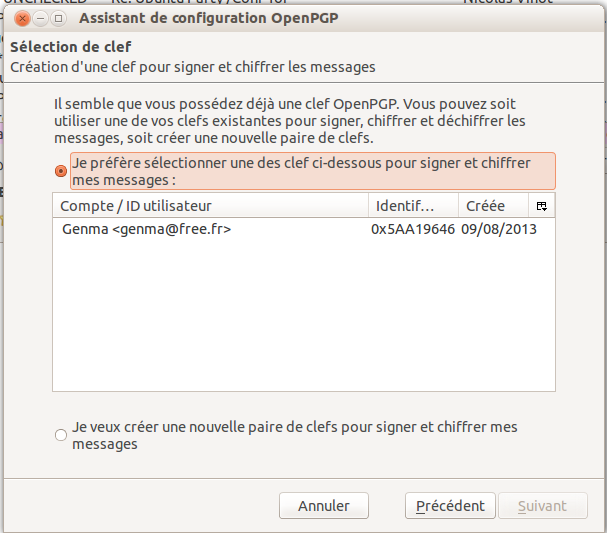
\includegraphics[scale=0.3] {./images/Assistant05.png}
\end{center}
\end{frame}

%----------------------------------------------------------------------------------------
\begin{frame}
\frametitle{Enigmail - l'assistant}
\begin{center}
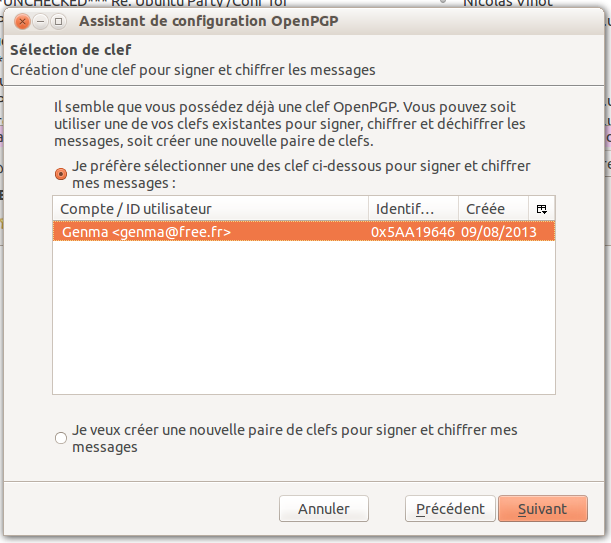
\includegraphics[scale=0.3] {./images/Assistant06.png}
\end{center}
\end{frame}

%----------------------------------------------------------------------------------------
\begin{frame}
\frametitle{Enigmail - l'assistant}
\begin{center}
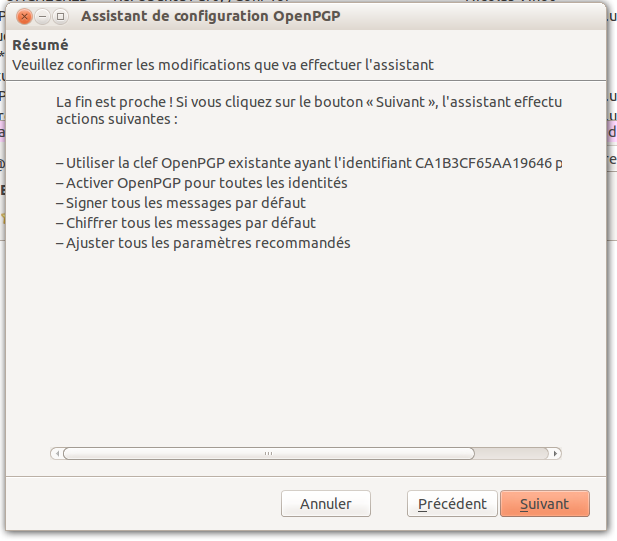
\includegraphics[scale=0.3] {./images/Assistant07.png}
\end{center}
\end{frame}

%----------------------------------------------------------------------------------------
\begin{frame}
\frametitle{Enigmail - l'assistant}
\begin{center}
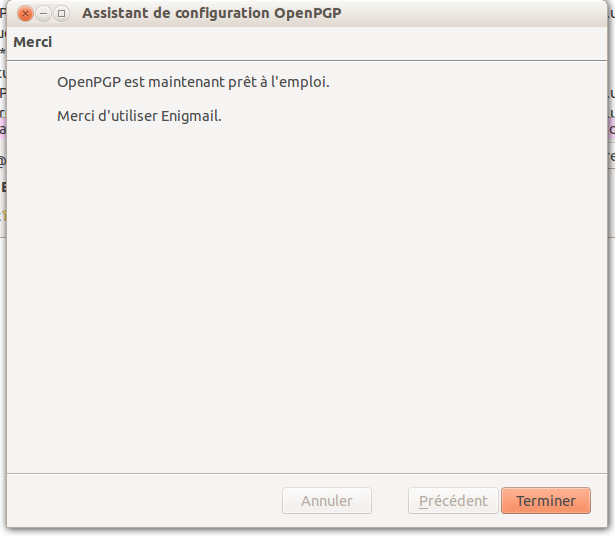
\includegraphics[scale=0.3] {./images/Assistant08.png}
\end{center}
\end{frame}

%----------------------------------------------------------------------------------------
\begin{frame}
\begin{center}
\Huge{Envoi d'un e-mail}
\end{center}
\end{frame}


%----------------------------------------------------------------------------------------
\begin{frame}
\frametitle{Thunderbird - création d'un mail chiffré}
\begin{center}
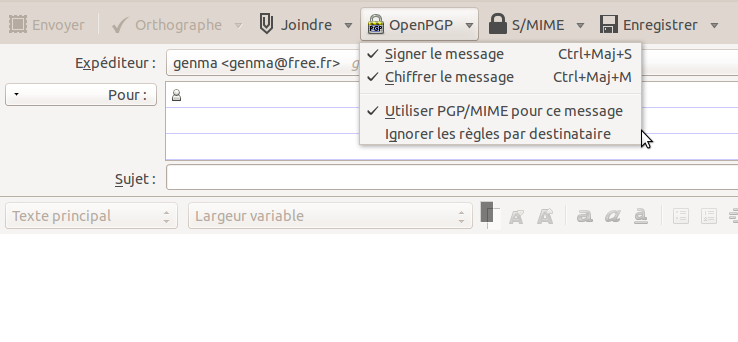
\includegraphics[scale=0.4] {./images/Thunderbird04.png}
\end{center}
\begin{itemize}
\justifying{
\item La création d'un mail dans Thunderbird se fait de la même façon qu'un e-mail classique.
\item Dans le menu OpenPGP, on peut choisir de signer le mail et/ou de le chiffrer.
}
\end{itemize}
\end{frame}


%----------------------------------------------------------------------------------------
\begin{frame}
\frametitle{Thunderbird - création d'un mail chiffré}
\begin{itemize}
\justifying{
\item La clef public du destinataire est utilisée en se basant sur son mail.
\item Il faut donc avoir sa clef avant d'envoyer le mail.
}
\end{itemize}
\end{frame}


\begin{frame}
\frametitle{Thunderbird - création d'un mail chiffré}
\begin{center}
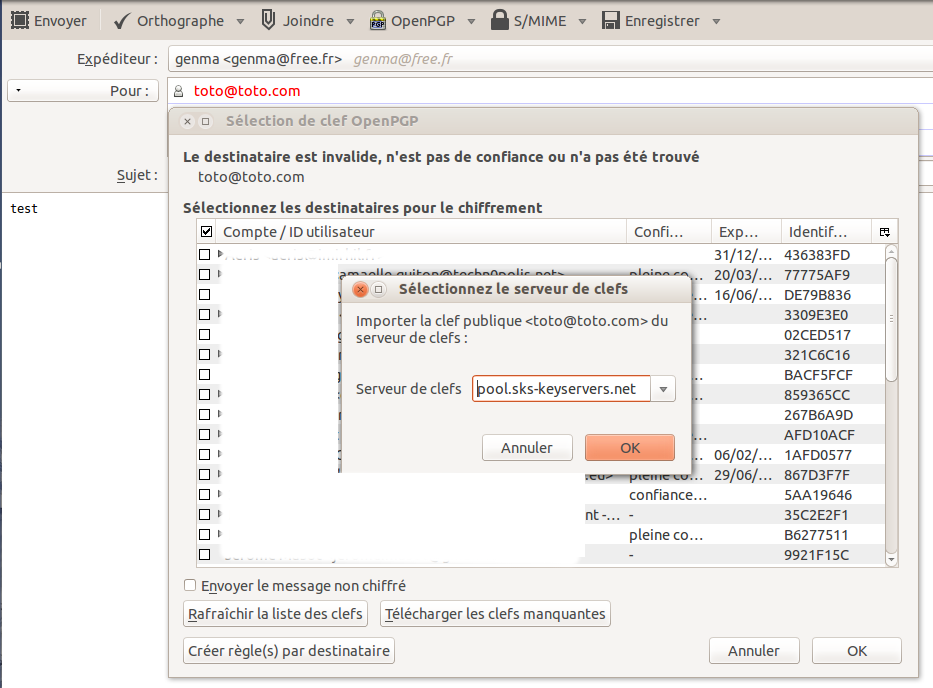
\includegraphics[scale=0.25] {./images/ClefInconnue.png}\end{center}
\begin{itemize}
\justifying{
\item Sinon, elle est automatiquement recherchée sur les serveurs de clefs.
}
\end{itemize}
\end{frame}


%----------------------------------------------------------------------------------------
\begin{frame}
\frametitle{Thunderbird - envoi/réception d'un mail chiffré}
\begin{center}
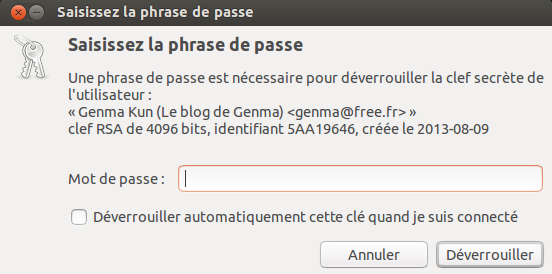
\includegraphics[scale=0.5] {./images/Thunderbird03.png}\end{center}
\begin{itemize}
\justifying{
\item A l'envoi du mail (cas où l'on signe) ou à la réception d'un mail chiffré, il est demandé de saisir son mot de passe de sa clef privée.
}
\end{itemize}
\end{frame}

%----------------------------------------------------------------------------------------
\begin{frame}
\frametitle{Webmail et mail chiffré}
\begin{center}
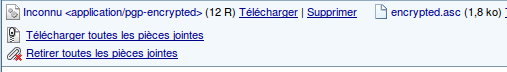
\includegraphics[scale=0.5] {./images/Zimbra.png}\end{center}
\end{frame}


%----------------------------------------------------------------------------------------
\begin{frame}
\begin{center}
\Huge{Enigmail - menus ajoutés dans Thunderbid}
\end{center}
\end{frame}

%----------------------------------------------------------------------------------------
\begin{frame}
\frametitle{Enigmail - menus ajoutés dans Thunderbid}
\begin{center}
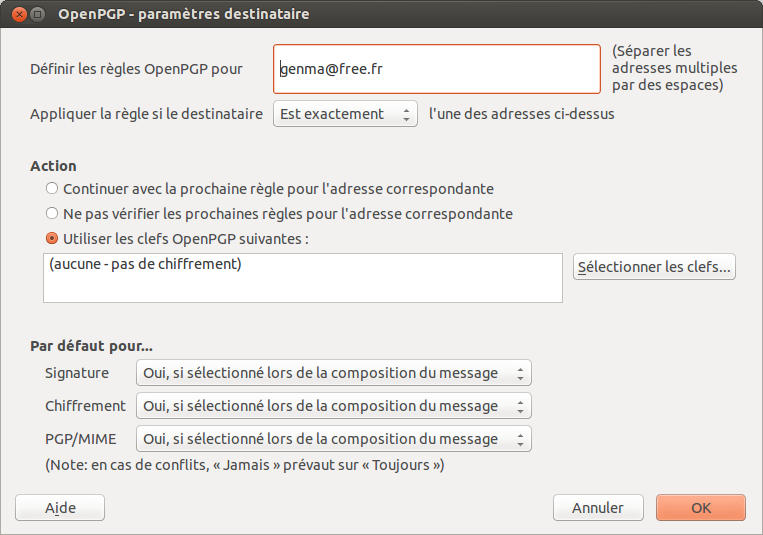
\includegraphics[scale=0.3] {./images/Enigmail01.png}
\end{center}
\end{frame}

%----------------------------------------------------------------------------------------
\begin{frame}
\frametitle{Enigmail - menus ajoutés dans Thunderbid}
\begin{center}
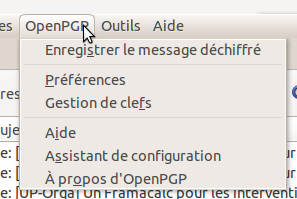
\includegraphics[scale=0.3] {./images/Menu_Options.png}
\end{center}
\end{frame}


%----------------------------------------------------------------------------------------
\begin{frame}
\frametitle{Enigmail - les préférences}
\begin{center}
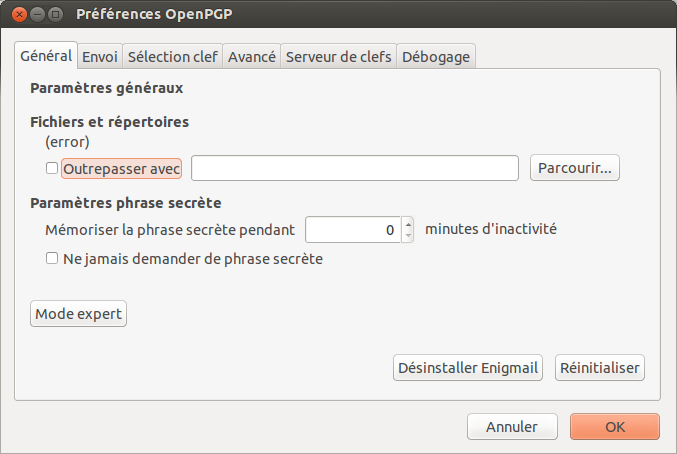
\includegraphics[scale=0.3] {./images/Enigmail02.png}
\end{center}
\end{frame}

%----------------------------------------------------------------------------------------
\begin{frame}
\frametitle{Enigmail - les préférences}
\begin{center}
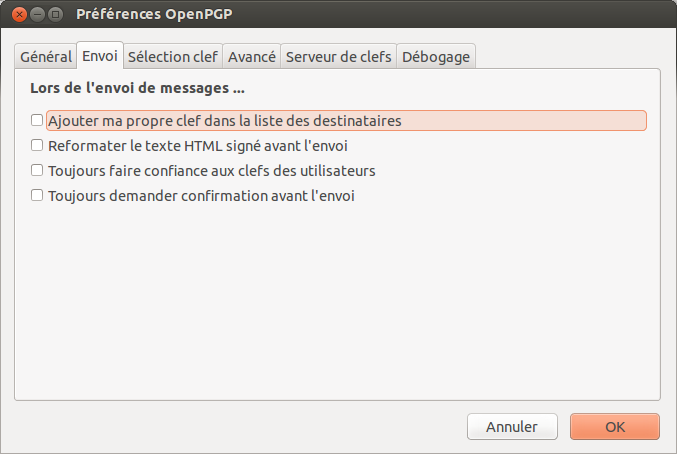
\includegraphics[scale=0.3] {./images/Enigmail03.png}
\end{center}
\end{frame}

%----------------------------------------------------------------------------------------
\begin{frame}
\frametitle{Enigmail - les préférences}
\begin{center}
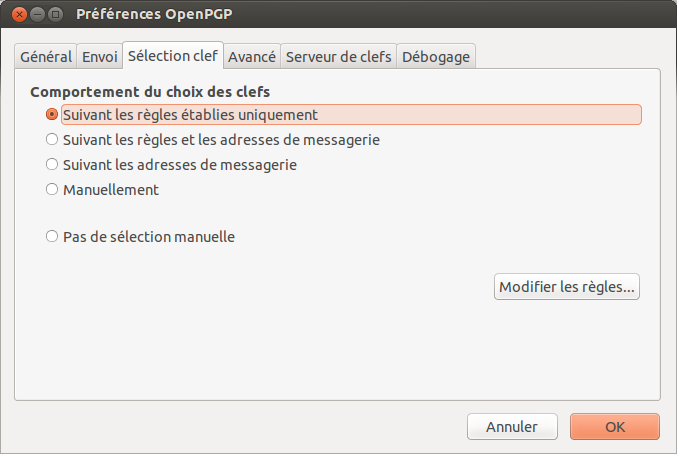
\includegraphics[scale=0.3] {./images/Enigmail04.png}
\end{center}
\end{frame}


%----------------------------------------------------------------------------------------
\begin{frame}
\frametitle{Enigmail - les préférences}
\begin{center}
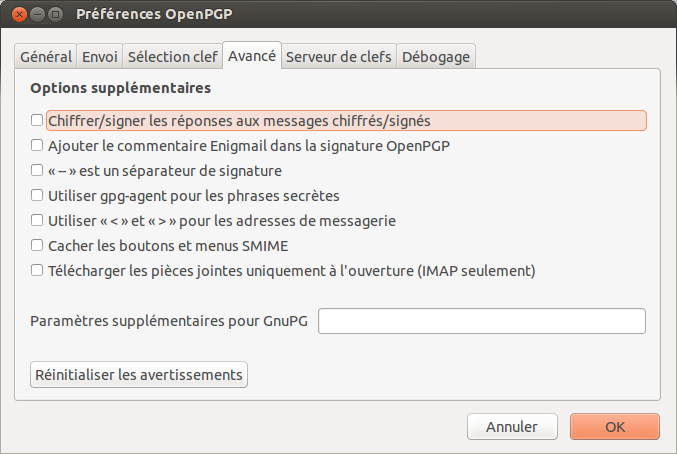
\includegraphics[scale=0.3] {./images/Enigmail05.png}
\end{center}
\end{frame}

%----------------------------------------------------------------------------------------
\begin{frame}
\frametitle{Enigmail - les préférences}
\begin{center}
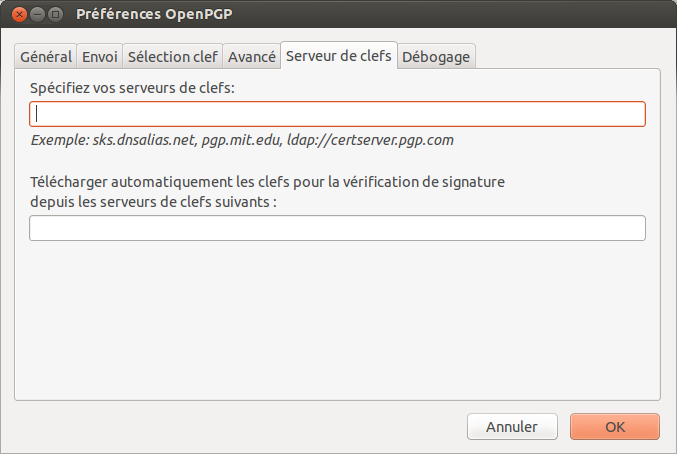
\includegraphics[scale=0.3] {./images/Enigmail06.png}
\end{center}
\end{frame}

%----------------------------------------------------------------------------------------
\begin{frame}
\frametitle{Enigmail - les préférences}
\begin{center}
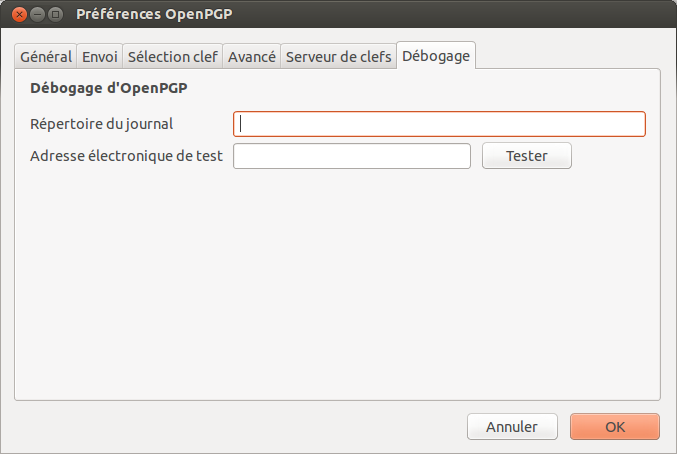
\includegraphics[scale=0.3] {./images/Enigmail07.png}
\end{center}
\end{frame}

%----------------------------------------------------------------------------------------
\begin{frame}
\begin{center}
\Huge{Questions - Démonstration }
\end{center}
\end{frame}
\end{document}


\end{document}
